\chapter{Implementation}
\section{Plans}


Nearing the end of every spring, the customer and group agreed upon the content of the following sprint. 


\begin{tabular}{|c|c|p{6cm}|}
\hline
Sprint nr. & Date & Summary\\
\hline
Sprint 1: & 03.02.13 - 08.02.13 & Developing user stories and paper prototypes of the GUI.\\ 
\hline
Sprint 2: & 08.02.13 - 15.02.13 & Developing a mock-up application demonstrating the GUI.\\
\hline
Sprint 3: & 15.02.13 - 22.02.13 & Improving UI and functionality for the prototype, researching medicinal factors. \\
\hline

\end{tabular} 

 

\section{Results}
\subsection*{Second mockup}
After the second meeting with the customer, the group had a sketch that was to be used as a starting point for the mock-up application. \\
\setlength\fboxsep{0pt}
\setlength\fboxrule{1pt}
\fbox{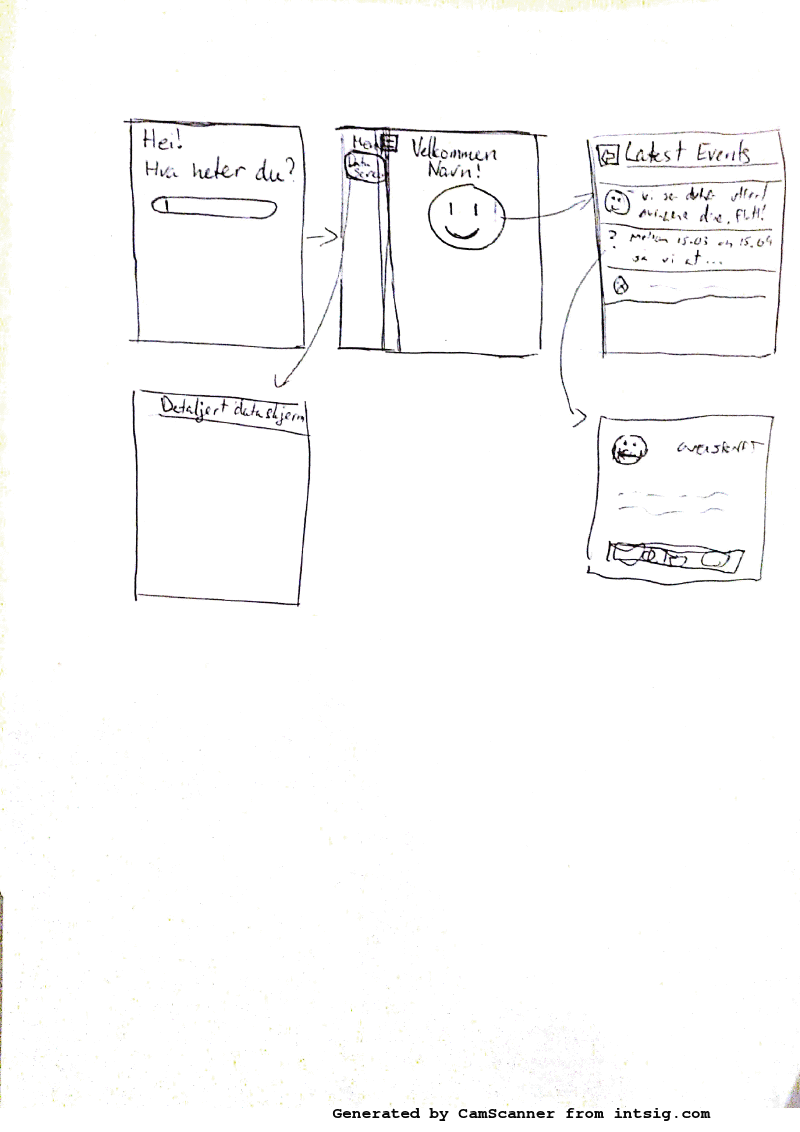
\includegraphics[trim = 20mm 180mm 0mm 20mm, clip, width=\linewidth]{Res/mockupV2}}


